\chapter{Using a command line and an editor}
\label{chp:cli}

In the first part of this book you used Jupyter notebooks as an interface to
Python. This has a number of advantages, the strongest of which is the ability
to include both code and prose in the same document. From this part of the book
onwards you will explore another approach to using Python which is to use 
a code editor and command line as a direct interface to your operating system.

\begin{note}
In this chapter you will cover:
\begin{itemize}
\item 

Using the cli.

\item 

Using an editor.

\end{itemize}
\end{note}





\section{Tutorial}

You will here consider a problem we have already solved in
Chapter~\ref{chp:algebra}
 but use a different interface to do so than Jupyter.
The code itself will be the same. The way you run it will differ.

Rationalise the denominator of \(\frac{1}{\sqrt{2} + 1}\)

Open a command line tool:

\begin{enumerate}

\item 

On \textbf{Windows} search for \texttt{Anaconda Prompt} (it should be available to you
after installing Anaconda). See Chapter~\ref{chp:using_notebooks}.

\item 

On \textbf{OS X} search for \texttt{terminal}. See
See Chapter~\ref{chp:using_notebooks}.


\end{enumerate}

Whether or not you are using the Windows or MacOS operating system 
changes the commands you need to
type. First, list the directory you are currently in:

On Windows:

\begin{cliin}
$ dir
\end{cliin}

On MacOS:

\begin{cliin}
$ ls
\end{cliin}

This is similar to using your file explorer to view the contents in a given
directory. Similarly to the way you double click on a directory in the file explorer
you
can navigate to a directory in the command line.

\begin{note}
Throughout this book, when there are commands to be typed in a command line
tool they will be prefixed with a \texttt{\$}. Do not type the \texttt{\$}.
\end{note}



To do this you use the same command on both operating systems \texttt{cd}.

You will do this to navigate to your \texttt{cfm} directoy. For example if, as in 
Chapter~\ref{chp:algebra}
 the \texttt{cfm} directory was put on the \texttt{Desktop}
directory you would run the following:

\begin{cliin}
$ cd Desktop
$ cd cfm
\end{cliin}

\begin{note}
The two statements are written under each other to denote that they are run
one after the other.
\end{note}

You will now create a new directory:

\begin{cliin}
$ mkdir scripts
\end{cliin}

Inside this directory you will run the same command as before to see the
contents:


On Windows:


\begin{cliin}
$ dir
\end{cliin}


On MacOS



\begin{cliin}
$ ls
\end{cliin}





If you have followed the steps described in Chapter~\ref{chp:using_notebooks}
will see something similar to Figure~\ref{fig:contents_of_directory_on_windows}
or Figure~\ref{fig:contents_of_directory_on_MacOS}.

\begin{figure}[htbp]
\centering
\noindent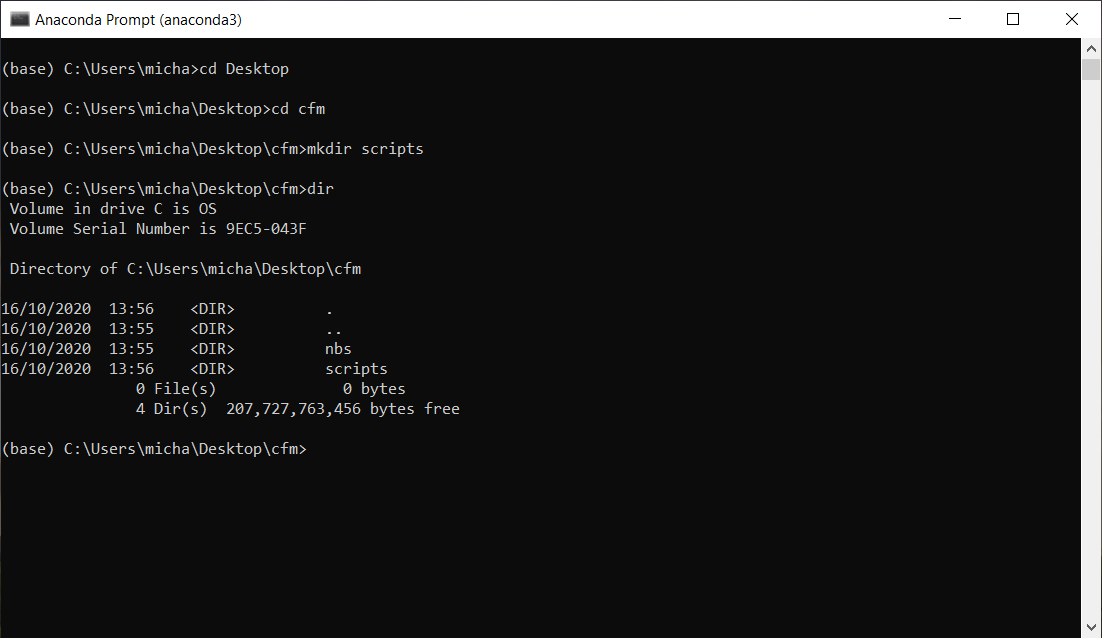
\includegraphics[width=0.750\linewidth]{./assets/output_of_dir/main.png}
\caption{The output of \texttt{dir} on Windows}
\label{fig:contents_of_directory_on_windows}
\end{figure}


\begin{figure}[htbp]
\centering
\noindent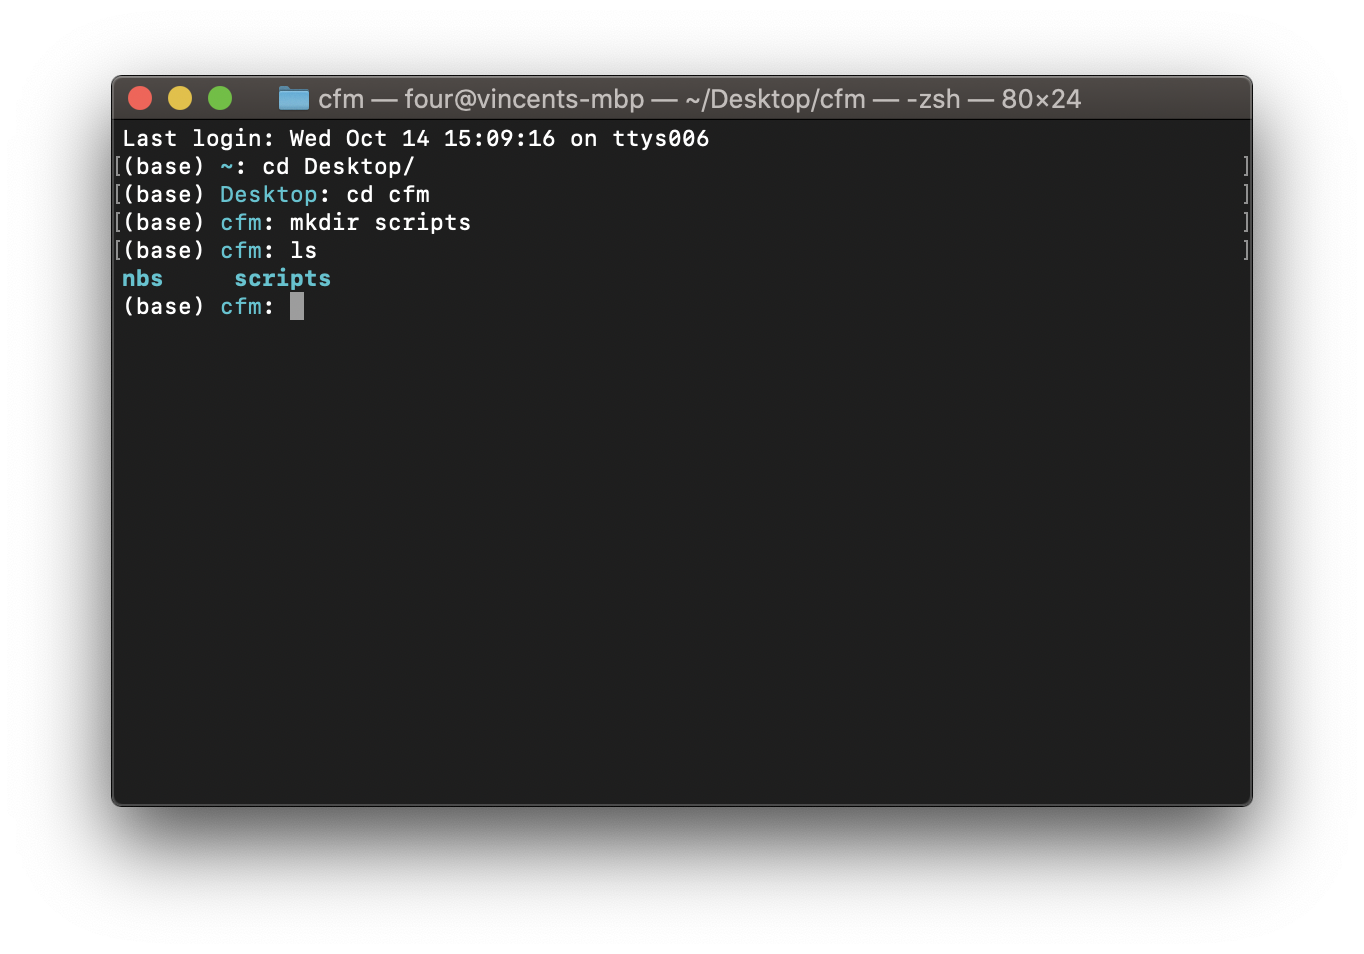
\includegraphics[width=0.750\linewidth]{./assets/output_of_ls/main.png}
\caption{The output of \texttt{ls} on MacOS}
\label{fig:contents_of_directory_on_MacOS}
\end{figure}


Before continuing with this directory you are going to install a
powerful code editor.
\begin{enumerate}

\item 

Navigate to \texttt{https://code.visualstudio.com}.

\item 

Download the installer making sure it is the correct one for your operating
system (Windows, MacOS or Linux).

\item 

Run the installer.

\end{enumerate}


This code editor will offer you a different way to write Python code.


Open VS code and create a new file.


In it write the following (which corresponds to the solution of our problem):

\begin{python}
"""
This script displays the solution to the problem considered.
"""
import sympy as sym

print("Question 1:")
expression = 1 / (sym.sqrt(2) + 1)
print(sym.simplify(expression))
\end{python}


This is shown in Figure~\ref{fig:code_in_vscode}.

\begin{figure}[!htbp]
\centering
\noindent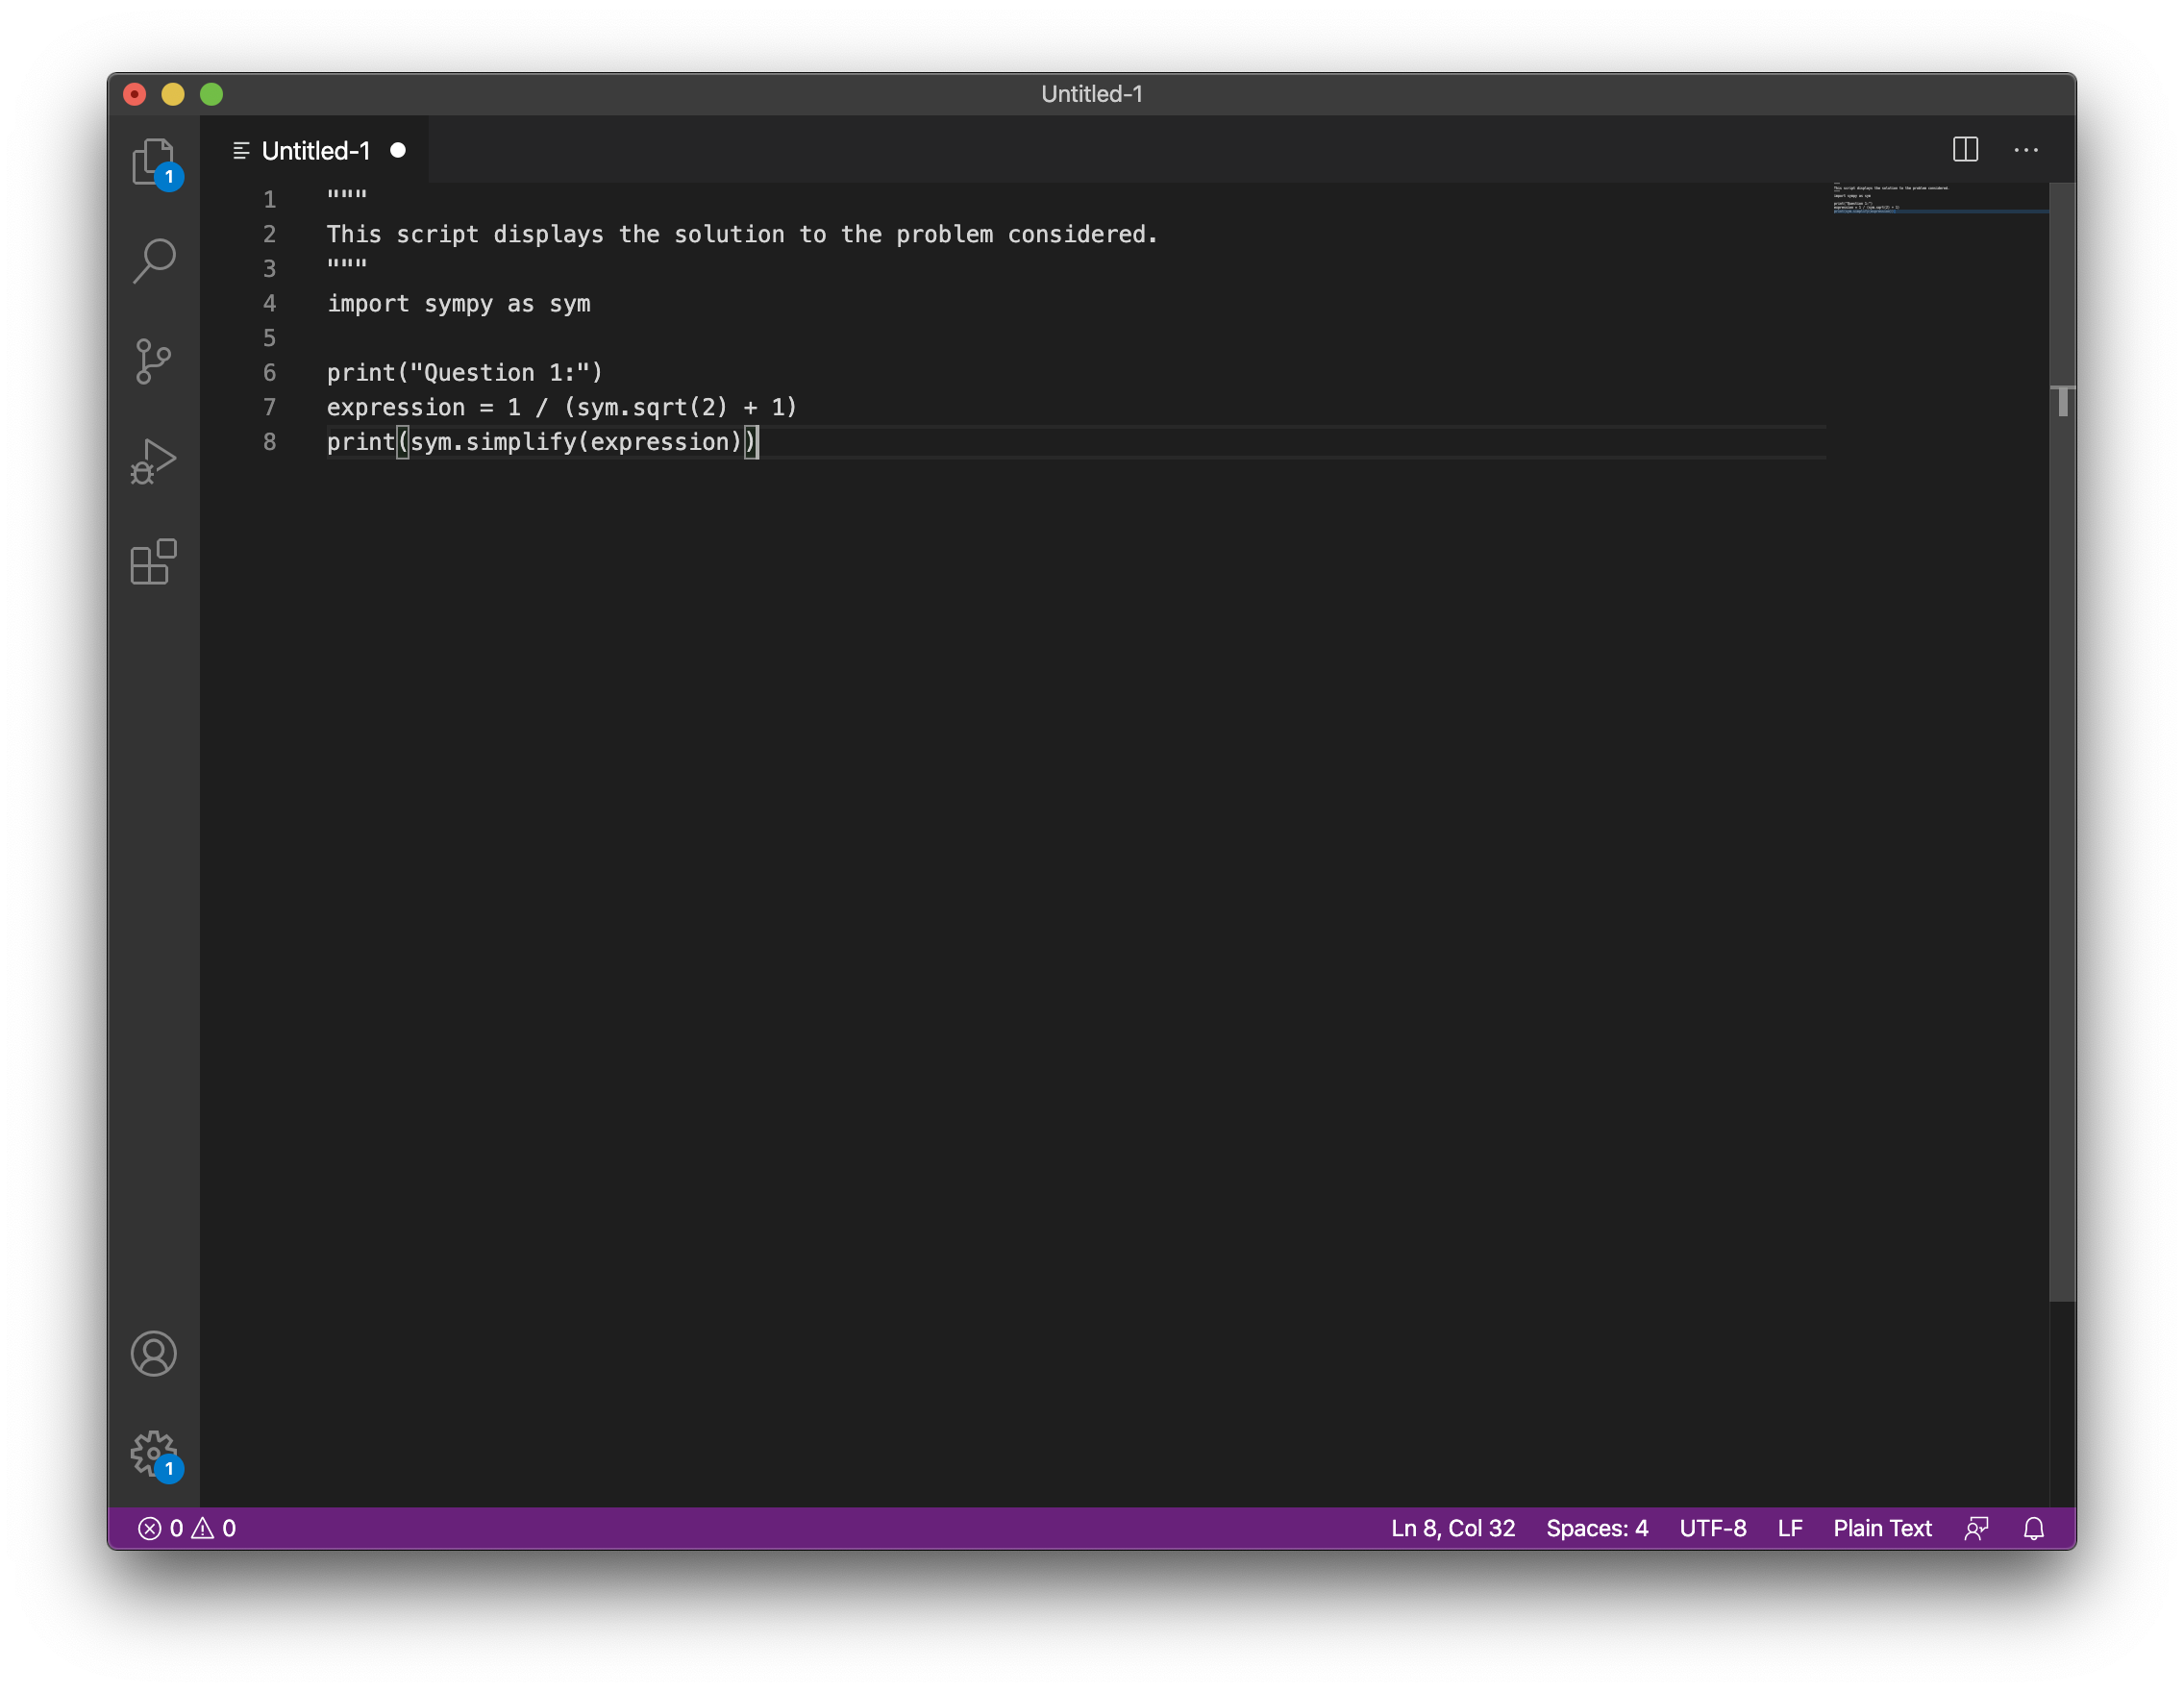
\includegraphics[width=0.750\linewidth]{./assets/code_in_vscode/main.png}
\caption{The code in VS code}
\label{fig:code_in_vscode}
\end{figure}


Now save this as \texttt{algebra.py} inside the \texttt{scripts} directory created
earlier as shown in Figure~\ref{fig:saving_file_in_vscode}.

\begin{figure}[!htbp]
\centering
\noindent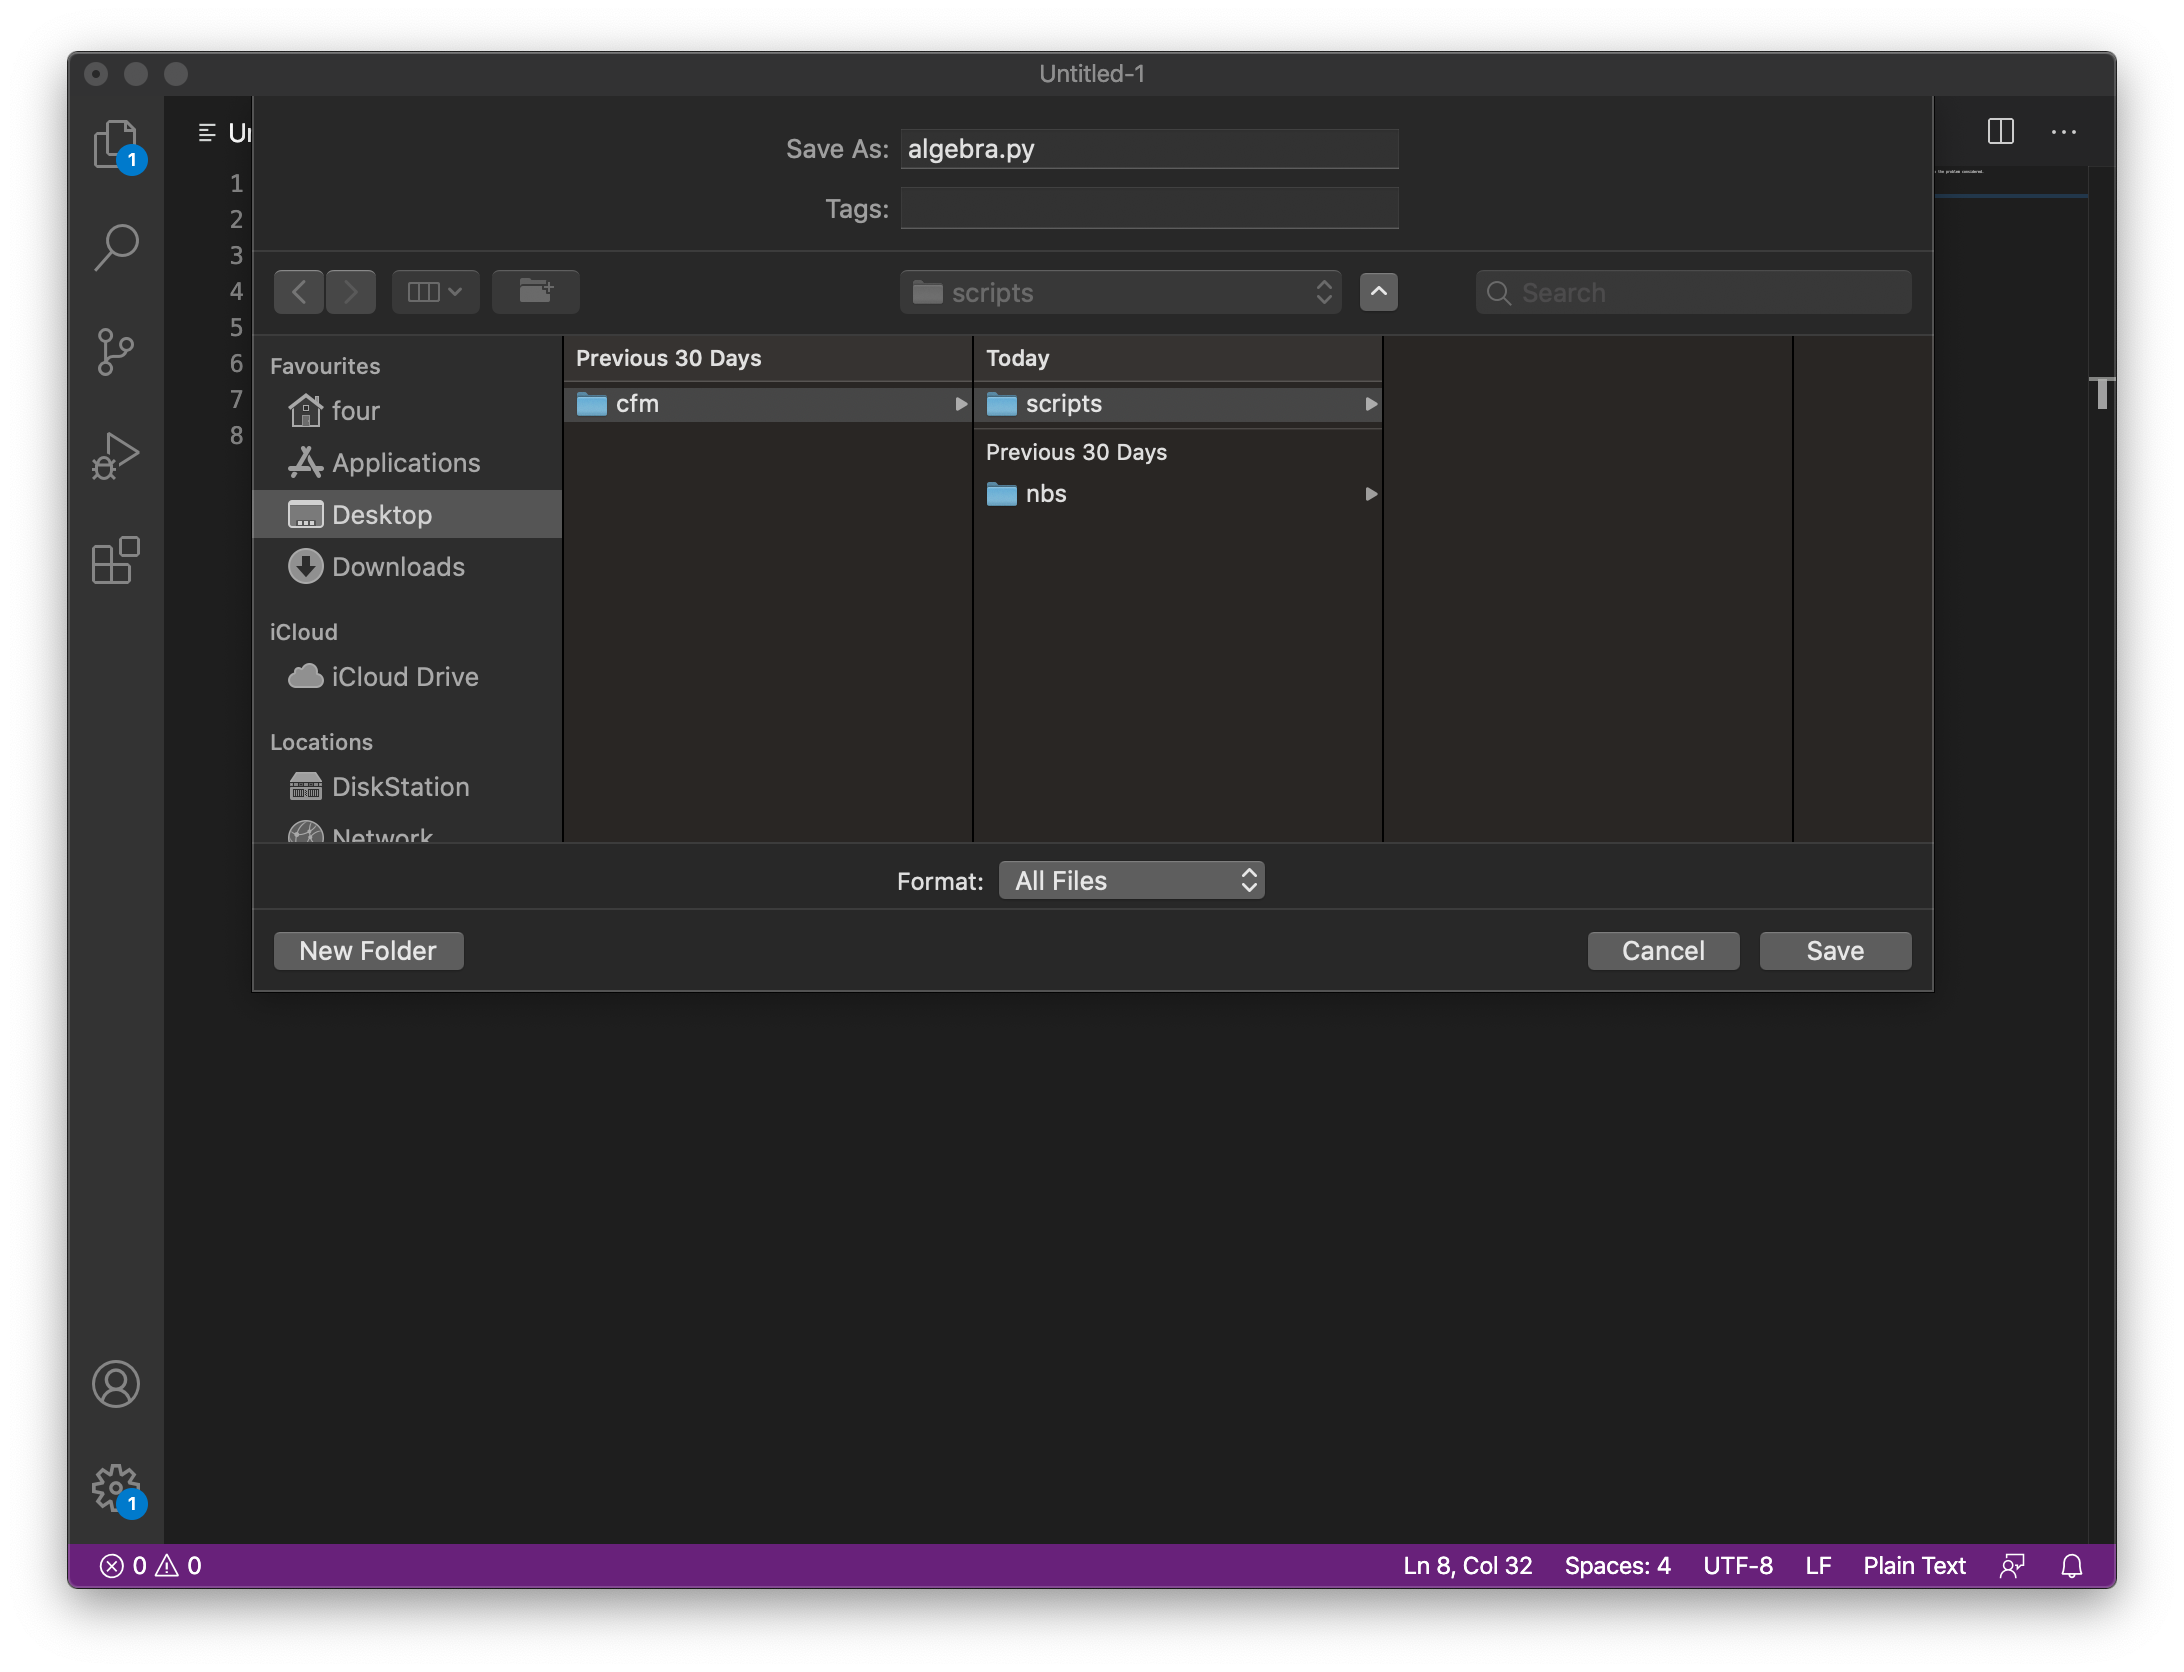
\includegraphics[width=0.750\linewidth]{./assets/saving_file_in_vscode/main.png}
\caption{Saving file in VScode}
\label{fig:saving_file_in_vscode}
\end{figure}


VScode now recognises the Python language and adds syntax colouring. It also
suggests a plugin specific for the Python language as shown in
Figure~\ref{fig:syntax_colouring_and_plugin_suggestion}. There is more information
about plugins in Section~\ref{sec:plugins_for_vs_code}.

\begin{figure}[!htbp]
\centering
\noindent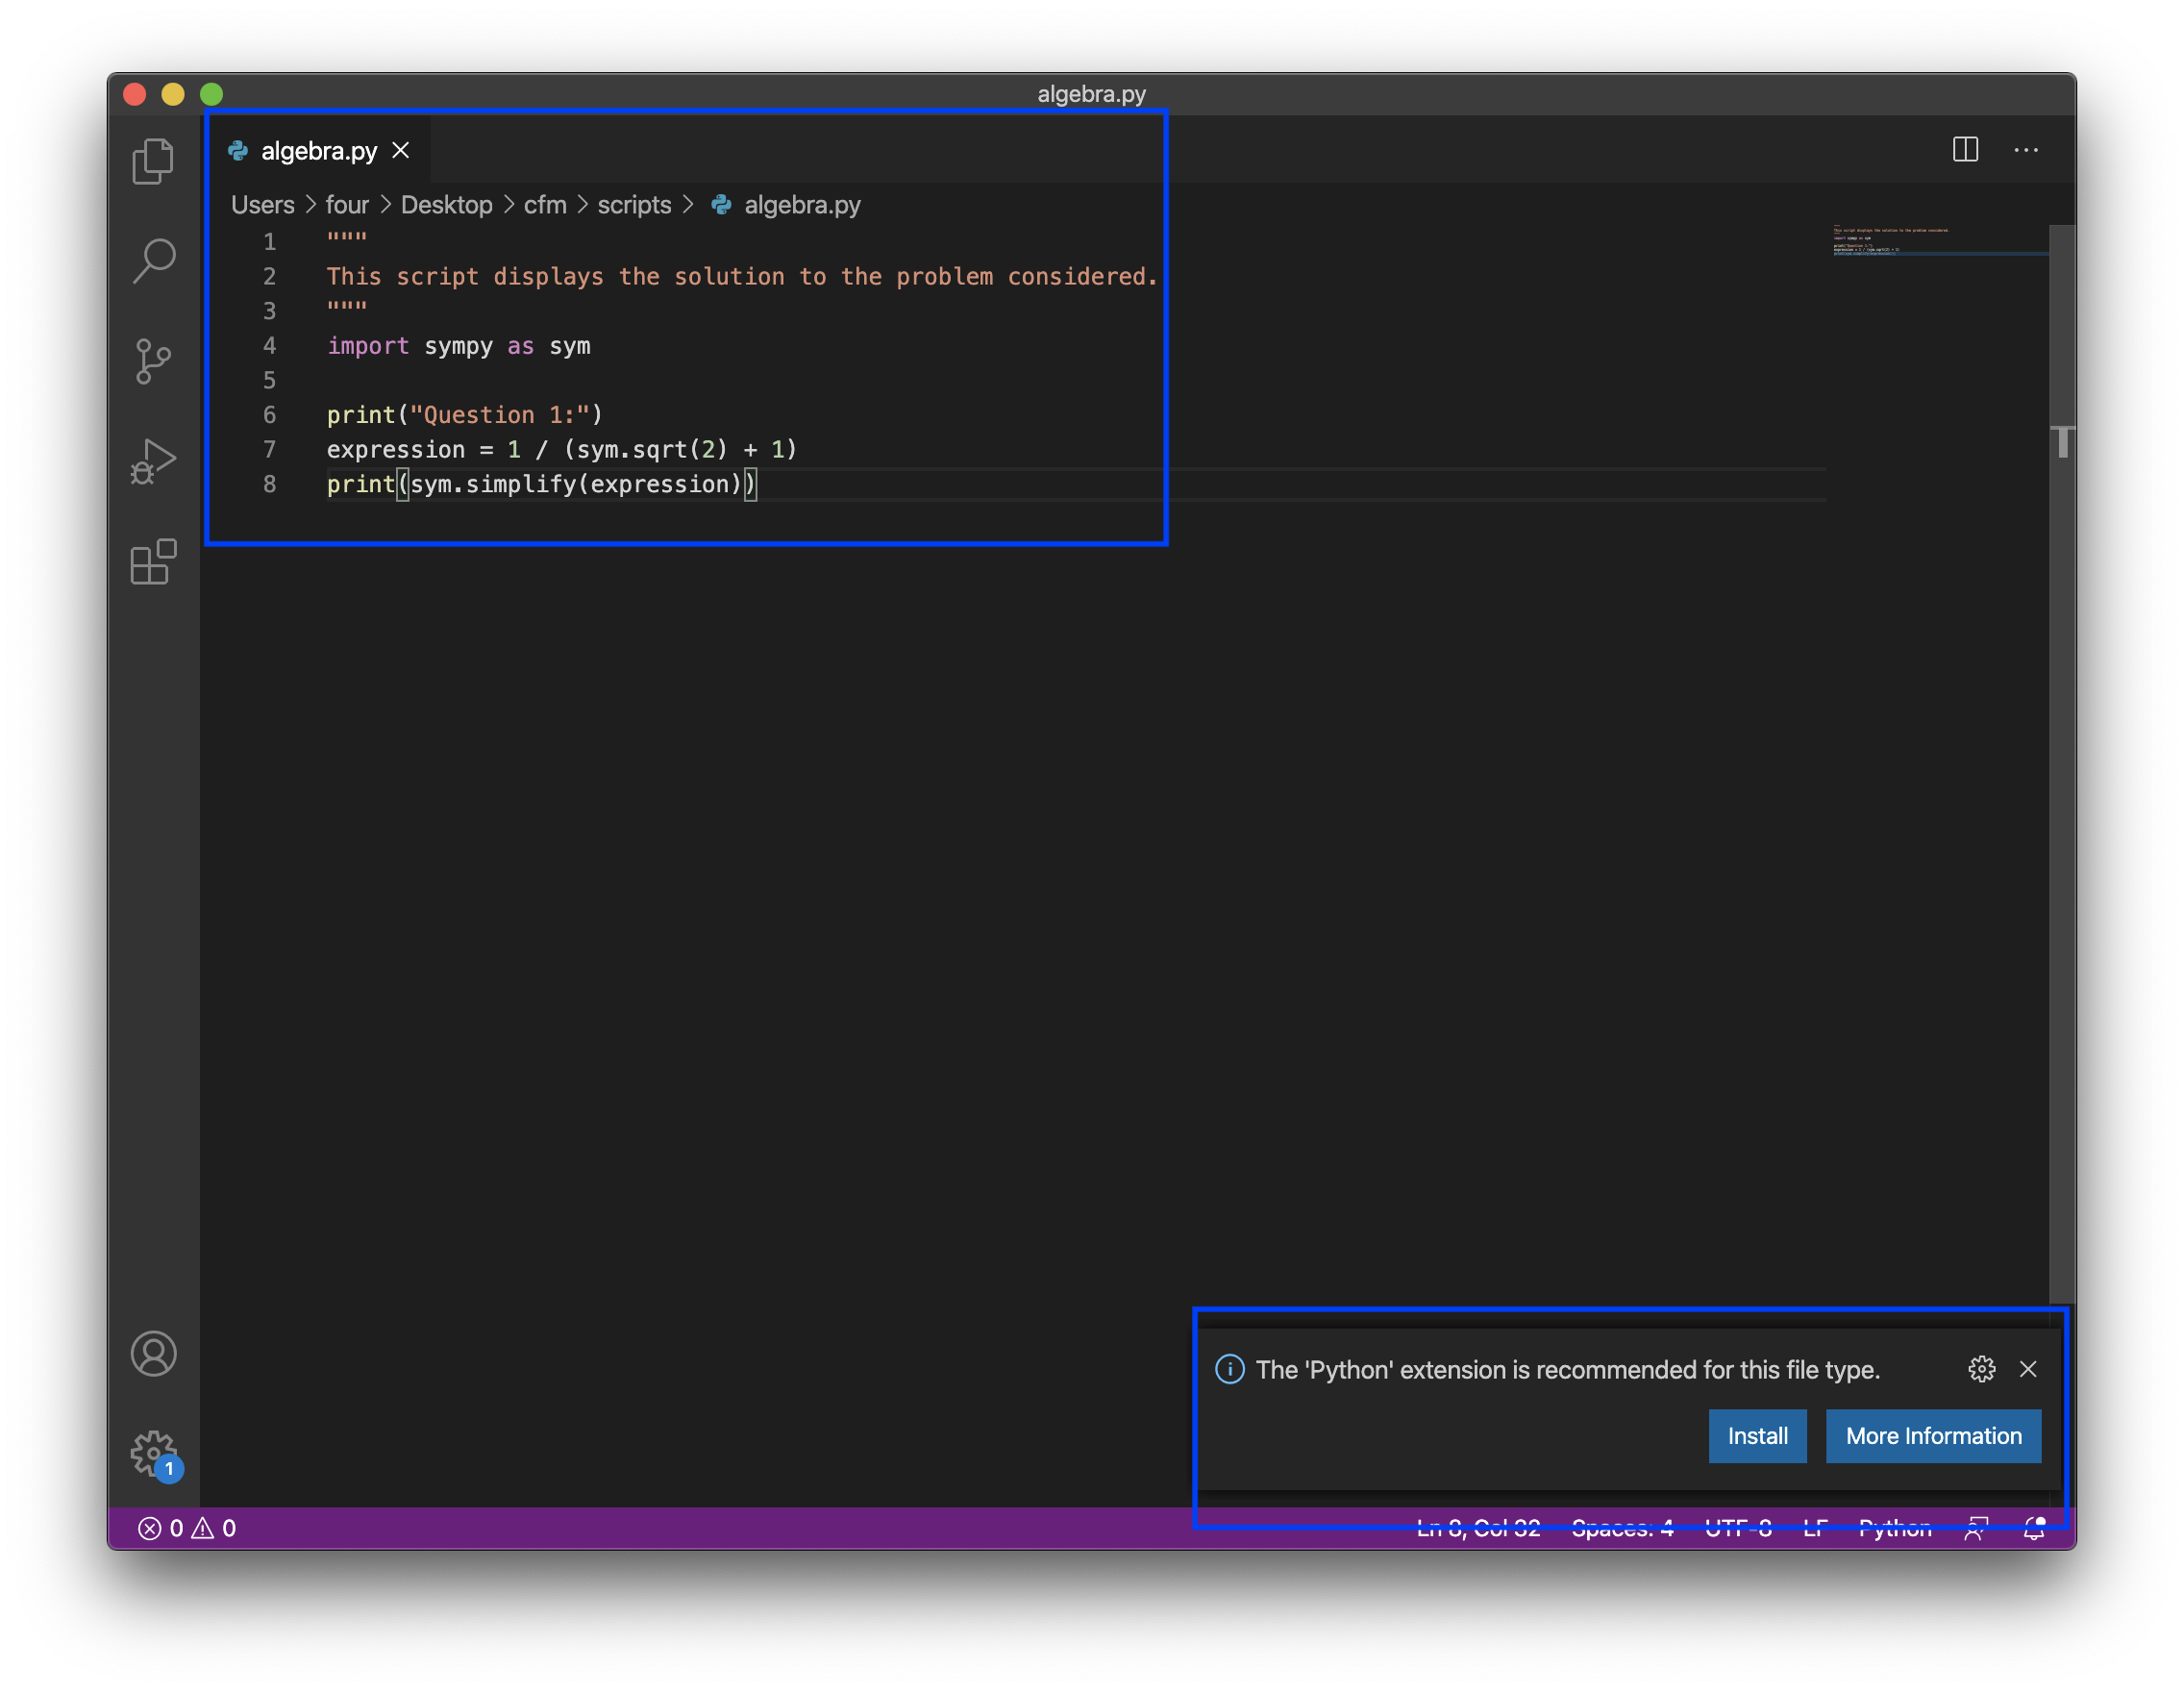
\includegraphics[width=0.750\linewidth]{./assets/syntax_colouring_and_plugin_suggestion/main.png}
\caption{Syntax colouring and plugin suggestion}
\label{fig:syntax_colouring_and_plugin_suggestion}
\end{figure}


All you have done so far is write the code. You now need to tell Python to run it.
To do this you will use the command line and run the same command on both operating systems:

\begin{cliin}
$ cd scripts
\end{cliin}


Now confirm that the \texttt{algebra.py} file is in that directory:


On Windows:


\begin{cliin}
$ dir
\end{cliin}



On MacOS:


\begin{cliin}
$ ls
\end{cliin}

Now run the python code in that script:

\begin{cliin}
$ python algebra.py
\end{cliin}


The output of this is shown in Figure~\ref{fig:output_of_running_script}


\begin{figure}[!htbp]
\centering
\noindent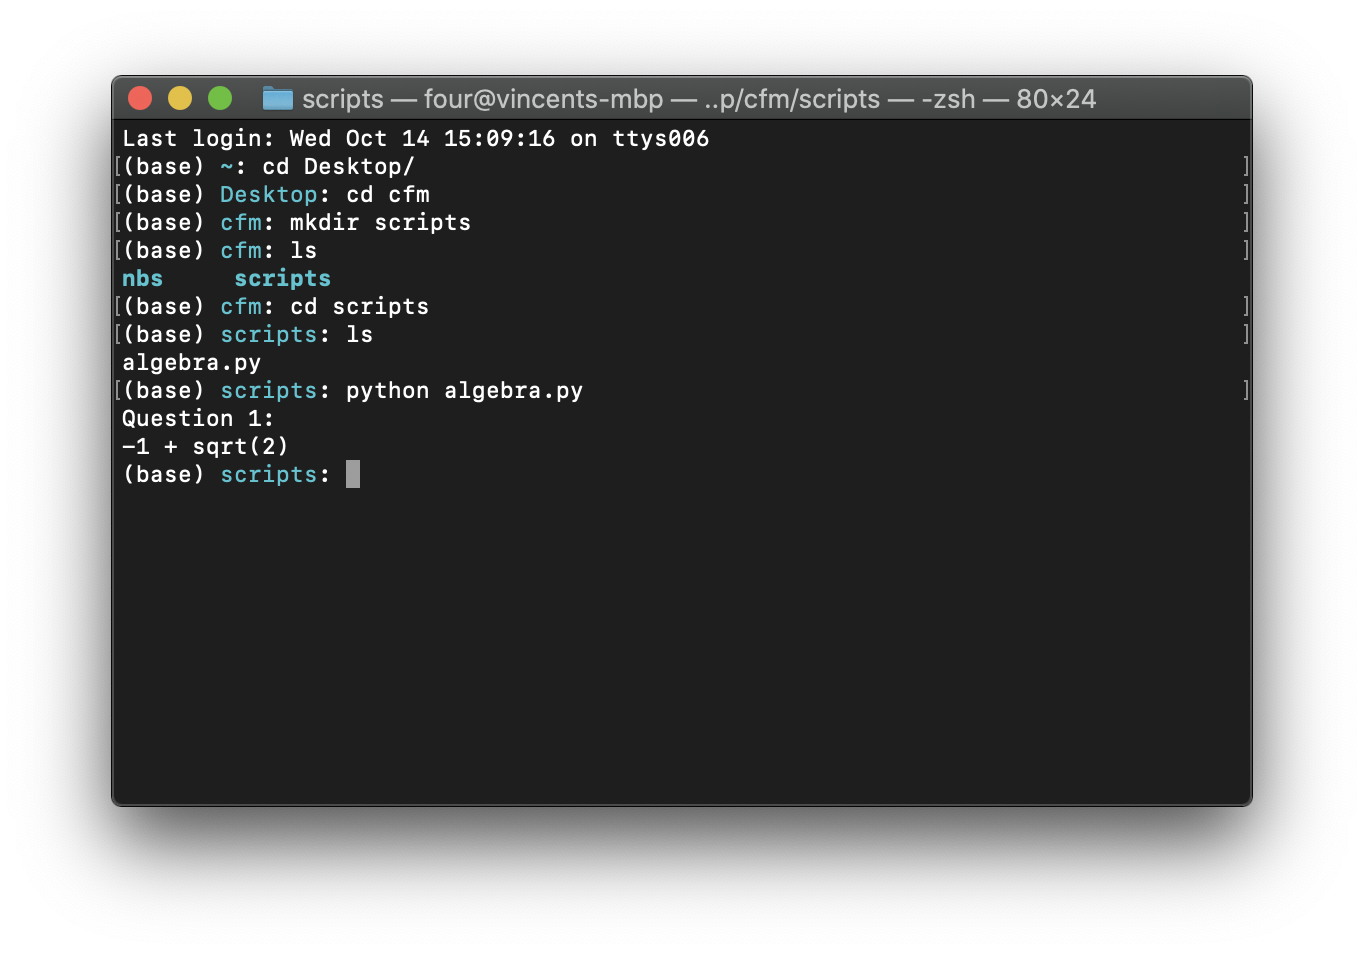
\includegraphics[width=0.750\linewidth]{./assets/output_of_running_script/main.png}
\caption{Output of running script}
\label{fig:output_of_running_script}
\end{figure}




\section{How to}

\subsection{Navigate directories using the command line}

In the command line the \texttt{cd} command (short for ``\texttt{c}hange \texttt{d}irectory'') can be
used to enter a given directory.

\begin{api}
$ cd <directory>
\end{api}


\begin{note}
The target directory must be contained in the directory you are currently in.
\end{note}

For example to change directory in to a directory called \texttt{cfm}:

\begin{cliin}
$ cd cfm
\end{cliin}

To go back to the previous directory use \texttt{..}:

\begin{cliin}
$ cd ..
\end{cliin}


\subsection{Create a new directory using the command line}
\label{\detokenize{building-tools/04-editor-and-cli/how/main:how-to-create-a-new-directory-in-the-command-line}}

In the command line the \texttt{mkdir} command (short for
``\texttt{m}a\texttt{k}e \texttt{dir}ectory``) can be
used to create a new directory.


\begin{api}
$ mkdir <directory>
\end{api}



For example to create a director called \texttt{scripts}:

\begin{cliin}
$ mkdir scripts
\end{cliin}


\subsection{See the contents of a directory in the command line}
\label{\detokenize{building-tools/04-editor-and-cli/how/main:how-to-see-the-contents-of-a-directory-in-the-command-line}}

In the command line we can see the contents of the current directory:
\begin{itemize}
\item 

On Windows using \texttt{dir}

\item 

On OS X using \texttt{ls}

\end{itemize}




\subsection{Run python code in a file}

To run code in a file type \texttt{python} followed by the name of the file in the
command line.


\begin{api}
$ python <file.py>
\end{api}

For example to run code in a file called \texttt{main.py}:

\begin{cliin}
$ python main.py
\end{cliin}


\subsection{Run python code without using a file or Jupyter}
\label{\detokenize{building-tools/04-editor-and-cli/how/main:how-to-run-python-code-without-using-a-file-or-jupyter}}

At the command line if you type \texttt{python} without passing a filename this will
create a prompt in which you can directly write Python code.


\begin{cliin}
$ python
\end{cliin}



When doing this, you see a prompt appear with \texttt{>>>}, you can directly type python
code in there and press enter:

\begin{raw}
>>> 2 + 2
4
\end{raw}

\begin{note}
This interface to Python is called a Read-Eval-Print-Loop and is often referred
to as a REPL.
\end{note}

\begin{note}
Using \texttt{python} is the simplest of python REPLs, there are others (for example
\texttt{ipython}).
\end{note}



This interface to Python is quite limited and should only be used for quick
access to Python as a way to run simple commands.



\subsection{Install VScode plugins}
\label{sec:plugins_for_vs_code}

VScode is a powerful editor with a number of plugins for different languages and
functionalities.


To install a particular plugin in the menu bar, click on \texttt{Code > Preferences > Extensions}.


From there you can search for a specific plugin and install it by clicking on
the install button.

\section{Exercises}
\label{\detokenize{building-tools/04-editor-and-cli/exercises/main:exercises}}\label{\detokenize{building-tools/04-editor-and-cli/exercises/main::doc}}

\begin{enumerate}
\item 

Use the REPL (read eval print loop) to carry out the following calculations:
\begin{enumerate}

\item 

\(3 + 8\)

\item 

\(3 / 7\)

\item 

\(456 / 21\)

\item 

\(\frac{4 ^ 3 + 2}{2\times 5} - 5 ^ {\frac{1}{2}}\)

\end{enumerate}

\item 

Install the Python plugin for VScode.

\item 

Use the command line and a python script written in VScode to solve the
following problems:
\begin{enumerate}

\item 

Find the solutions to the following equation: \(x ^ 2 - 3 x + 2 = 1\).

\item 

Differentiate the following function: \(f(x) = \cos(x) / 4\)

\item 

Find the determinant of \(A = \begin{pmatrix} 1 / 5 & 1\\1 & 1\end{pmatrix}\).

\item 

Count the number of ways of picking 2 letters from “ABCD” where order
does not matter.

\item 

Simulate the probability of picking a red token from a bag with 3 red
rokens, 5 blue tokens and a yellow token.

\item 

Obtain the first 5 terms of the sequence defined by:
\begin{equation*}
\begin{split}
        \left\{
            \begin{array}{l}
              a_0 = 0,\\
              a_1 = 2,\\
              a_n = 3 a_{n - 1} + a_{n - 2}, n \geq 2
            \end{array}
        \right.
      \end{split}
\end{equation*}
\end{enumerate}

\item 

Install the \texttt{Markdown all in one} plugin for markdown in VScode and then:
\begin{enumerate}

\item 

Create a new file \texttt{main.md}.

\item 

Write some basic markdown in it.

\item 

Use the plugin to preview the rendered markdown.

\end{enumerate}

\end{enumerate}




\section{Further information}
\label{\detokenize{building-tools/04-editor-and-cli/why/main:further-information}}\label{\detokenize{building-tools/04-editor-and-cli/why/main::doc}}

\subsection{Why do you need to use the \texttt{print} function with an editor?}
\label{\detokenize{building-tools/04-editor-and-cli/why/main:why-do-we-need-to-use-the-print-function-with-an-editor}}

When using a Jupyter notebook, the last line of a cell corresponds to the
output of the cell and is automatically displayed.
When running code written in an editor directly through the Python interpreter
there is nowhere for code to be output to. Thus, you need to specifically tell it
to display the code which is what the \texttt{print} statement does.


\subsection{Can you use a Python plugin to run my code from inside my editor?}
\label{\detokenize{building-tools/04-editor-and-cli/why/main:can-i-use-a-python-plugin-to-run-my-code-from-inside-my-editor}}

When using the Python plugin buttons become available that let you run code
without using the command line. Before using those buttons it is good to become comfortable using a
command line tool to fully understand what the underlying process is. Furthermore,
at times when debugging sometimes the user interface might be at fault.


\subsection{Can I open a Jupyter notebook inside vscode?}
\label{\detokenize{building-tools/04-editor-and-cli/why/main:can-i-open-a-jupyter-notebook-inside-vscode}}

When using the Python plugin it is actually possible to use Jupyter notebooks
from within VScode.
The notebooks will not look exactly the same but have the same functionality as
shown in Figure~\ref{fig:a_notebook_in_vscode}.

\begin{figure}[htbp]
\centering
\noindent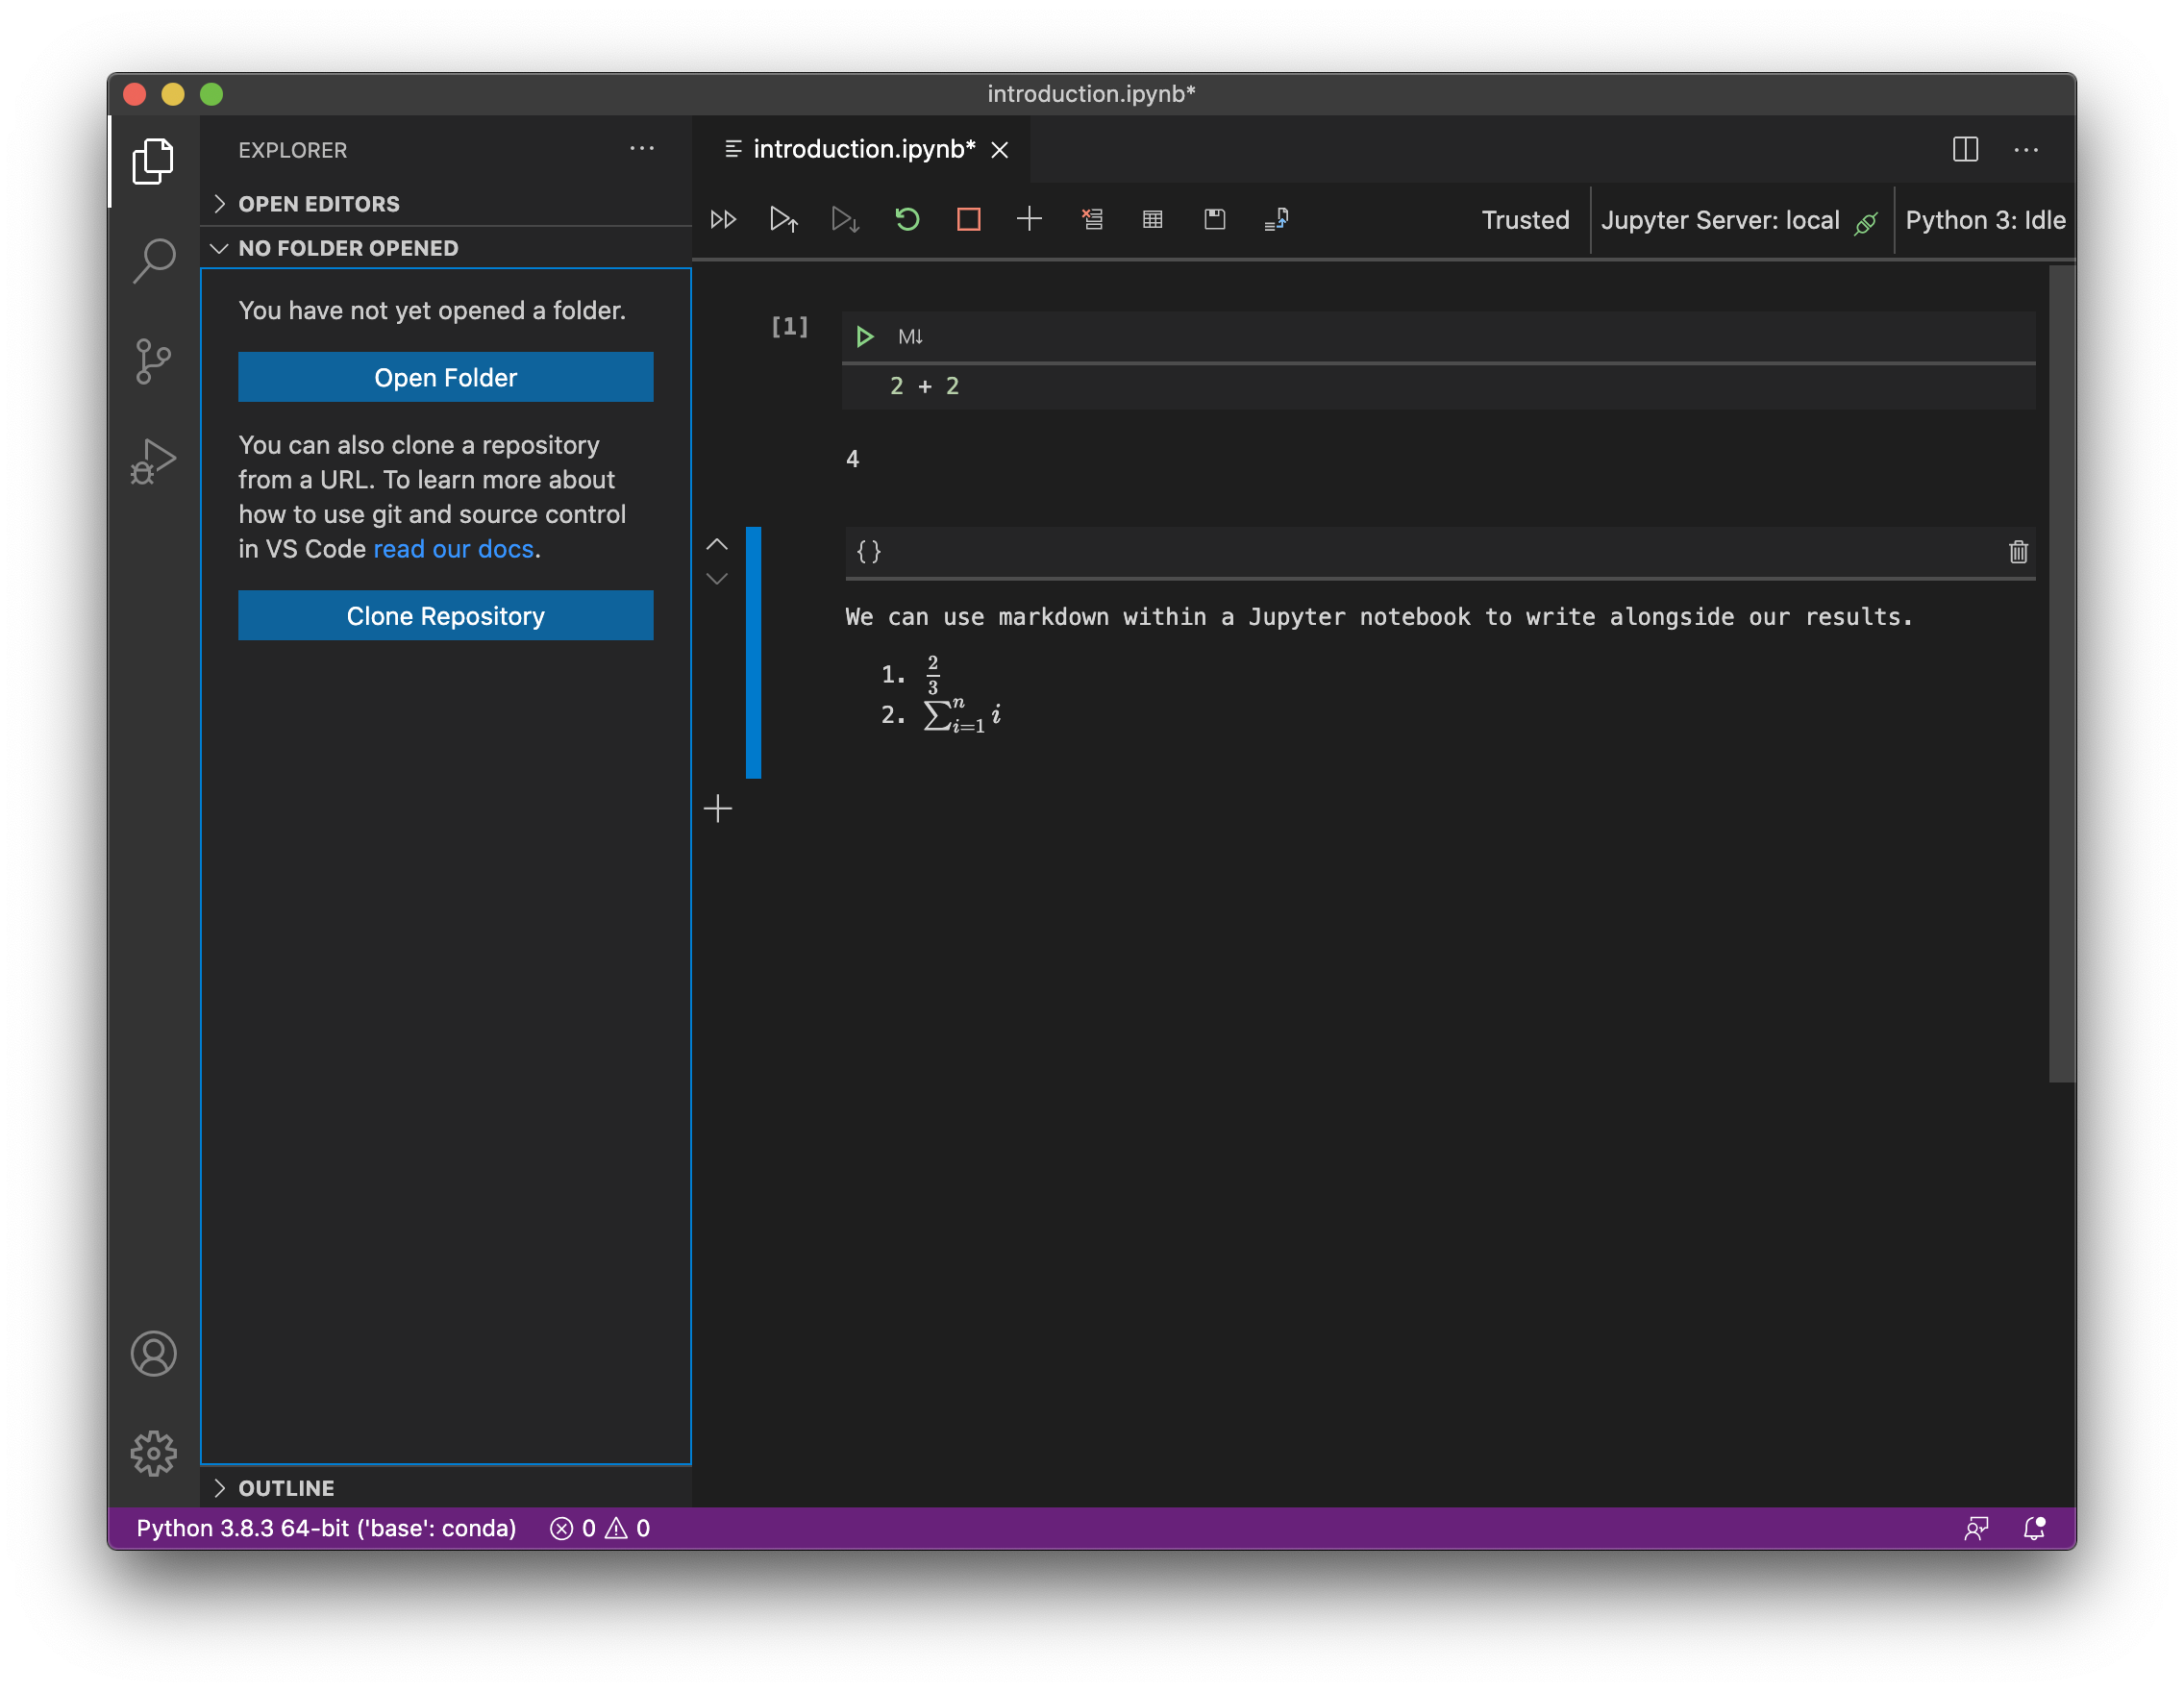
\includegraphics[width=0.750\linewidth]{./assets/notebook_in_vscode/main.png}
\caption{A notebook in vscode}
\label{fig:a_notebook_in_vscode}
\end{figure}


\subsection{What is the difference between an Integrated Development Environment and an editor?}
\label{\detokenize{building-tools/04-editor-and-cli/why/main:what-is-the-difference-between-an-integrated-development-environment-and-an-editor}}

An \textbf{I}ntegrated \textbf{D}evelopment \textbf{E}nvironment or IDE is another type of tool used
to write code. A popular one for Python is PyCharm.
Generally IDEs are powerful tools designed for one specific language whereas
editors are supposedly lightweight and designed to be flexible to be used with
many languages.


Experiment with IDEs and/or editors to find what you prefer but
throughout this book VSCode.


\subsection{Can I use \texttt{\textbackslash(} and \texttt{\textbackslash)} instead of \texttt{\$} for \LaTeX?}

When using Jupyter notebooks (see Section~\ref{sec:can_i_use_different_latex_delimiters_in_latex}) or the markdown preview feature in VScode the
single \texttt{\$} and \texttt{\$\$} must be used as delimiters for mathematics.
